%
% $XORP: xorp/docs/user_manual/livecd.tex,v 1.1 2005/04/11 23:28:02 pavlin Exp $
%

\chapter{XORP Live CD}
\label{livecd}

The XORP Live CD is a bootable CD for x86 PCs.
The Live CD serves a number of purposes:

\begin{itemize}

  \item It's an easy way to try out XORP without needing to
  compile anything or reformat the disk on your PC.
  \item It's a quick way to get a relatively secure router on demand.
  \item It's a great tool for a student lab session, requiring no
  installation.

\end{itemize}

See the XORP Web site ({\stt http://www.xorp.org/}) for information
how to download the lastest version of the XORP LiveCD ISO image.
Once you've downloaded the CD image, you will need to burn it using a
CD-R or CD-RW drive. For example, in case of FreeBSD you can simply run:

{\tt burncd -f /dev/acd0c -e data LiveCD.iso fixate}

See the XORP Web site for some URLs with instructions on how to burn CD images
on other systems.

\section{Running the Live CD}

To boot from the Live CD, your PC needs to have the CD-ROM device
set as the primary boot device.  If this is not already the case, you will
need to modify the settings in the BIOS.  The boot order should along the
lines of:

\begin{enumerate}
  \item CD drive.
  \item Floppy Disk.
  \item Hard Disk.
\end{enumerate}

The order of the floppy and hard disk are unimportant, just so
long as they're after the CD drive in the boot order.  This is usually
pretty easy to change in the BIOS - you might want to make a note of
the original boot order in case you want to switch it back afterwards.
Typically to change BIOS settings, you hold down Delete or F2
(depending on your PC) just after you restart your PC.

If you want the router to store any configuration changes you have made
when it is rebooted, you'll also need a floppy disk, but you can try
the Live CD without this.

Then reboot the PC.  The PC should boot from the CD.  Normally it will
display a low resolution XORP logo for 30 seconds to a minute while
booting completes.  Sorry - there's no progress bar to let you know
anything is happening.

If you've got a floppy in the floppy drive, and you've done this
before, then the XORP configuration will be copied into the memory
filesystem, along with passwords, sshd keys, etc.  Then the XORP
routing protocols will be started.

If there's no floppy in the drive, or it doesn't have the files on it
that XORP expects, then a simple interactive script will run to allow
you to configure passwords and decide which network interfaces you
want XORP to use.


\section{Starting XORP the First Time}

The startup script that runs the first time you run XORP is quite
simple. If there's no floppy in the floppy drive, or it's not
DOS-formatted, you'll be presented with a warning similar to the one in
Figure~\ref{fig:livecd:cd1}.

\begin{figure}[h]
  \begin{center}
    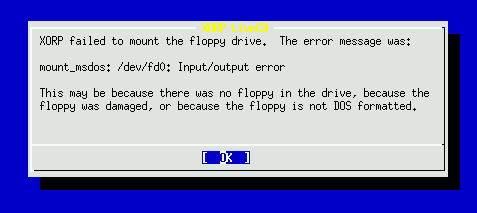
\includegraphics[width=6.0in]{figs/cd1}
    \caption{LiveCD missing floppy-related warning}
    \label{fig:livecd:cd1}
  \end{center}
\end{figure}

Hit enter, and you'll be given the choices shown in
Figure~\ref{fig:livecd:cd2}.

\begin{figure}[h]
  \begin{center}
    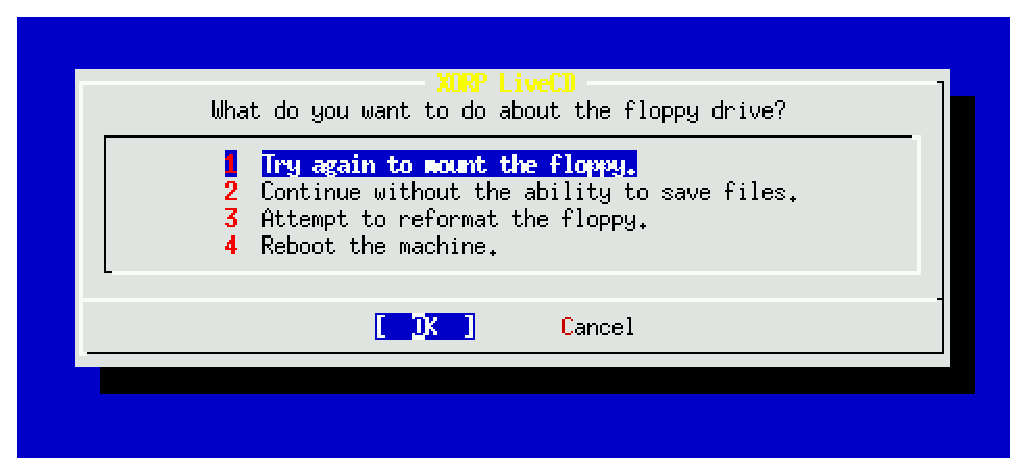
\includegraphics[width=6.0in]{figs/cd2}
    \caption{LiveCD floppy-related menu}
    \label{fig:livecd:cd2}
  \end{center}
\end{figure}


Use the cursor keys to move up and down to choose an option, and hit enter.

If you hadn't got a floppy in the drive, you can add one now, and select 1.

If your floppy is not DOS formatted, you can reformat it (erasing all the data
on it) by selecting 3.

If you don't have a floppy to hand, you can continue by selecting 2,
but you won't be able to preserve any configuration changes you make
later.

If you now have a blank writable DOS formatted floppy in the floppy
drive, you'll get the notice shown in Figure~\ref{fig:livecd:cd3}.

\begin{figure}[h]
  \begin{center}
    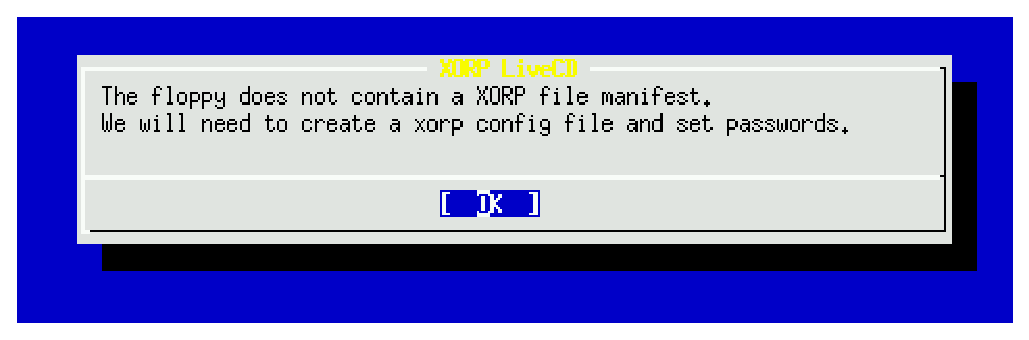
\includegraphics[width=6.0in]{figs/cd3}
    \caption{LiveCD floppy-related message}
    \label{fig:livecd:cd3}
  \end{center}
\end{figure}

Hit Enter, and you will be prompted to enter the root password for the
FreeBSD system.  This will allow you to login to the machine as the
superuser to diagnose any problems, or to see how XORP works behind
the scenes.

Next you will be prompted to enter the password for the "xorp" user
account.  On a normal XORP router, you might have many user accounts
for the different router administrators, but on the Live CD we just
create one user called "xorp".  Please do enter a reasonable password,
as this user will be able to login over the network using the ssh
secure shell and this password.

Finally you will be prompted as to which network interfaces you wish
XORP to manage.  These interfaces will show up in the default XORP
configuration file, ready to have IP addresses assigned.  The menu
looks like the one shown in Figure~\ref{fig:livecd:cd4}.

\begin{figure}[h]
  \begin{center}
    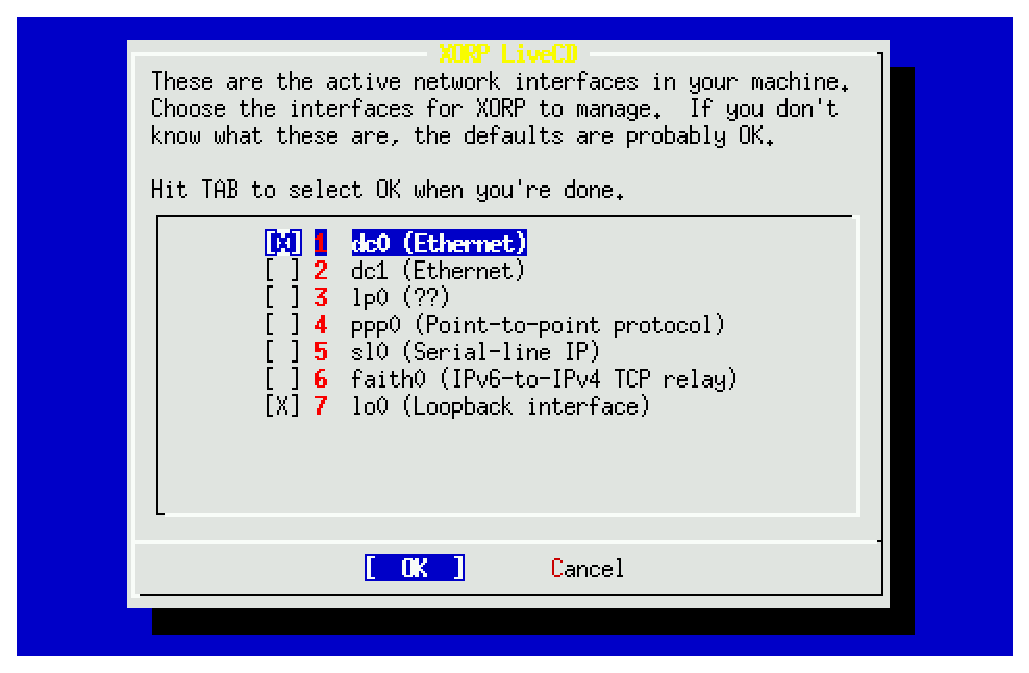
\includegraphics[width=6.0in]{figs/cd4}
    \caption{LiveCD network interfaces menu}
    \label{fig:livecd:cd4}
  \end{center}
\end{figure}

Typically you will only want XORP to manage Ethernet interfaces and
the loopback interface from the Live CD at this stage, because currently
XORP has no built-in support for dial-up links.  Move up and down using the
cursor keys, and hit space to select or unselect an option (an "X"
implies the option is selected).  When you are finished, hit Tab, to
select the "OK" button, and hit Enter.

That's it.  XORP will now finish booting.

Once XORP has finished booting, you will be presented with a login
prompt, and you can login to XORP as the "xorp" user with the password
you have chosen, and interact with the XORP command line interface to
complete the configuration, assign IP addresses, etc.

\section{Saving Config}

The location of the router configuration file used by XORP can be set
using command line parameters, so different XORP systems might choose
to use a different location for this file.  On the Live CD, the
configuration file is stored in {\stt /etc/xorp.cfg}.

If you change the router configuration using the XORP shell, and want
to save it, you need to enter the following in configuration mode:

\vspace{0.1in}
\noindent\framebox[\textwidth][l]{\scriptsize
\begin{minipage}{6in}
\begin{alltt}
\begin{tabbing}
xxxxxxxxxxxxxxxxxx\=\kill
user@hostname\# \textbf{save /etc/xorp.cfg}
\end{tabbing}
\end{alltt}
\end{minipage}
}
\vspace{0.1in}

If you save to any other location, the file will still be preserved on
the floppy, but will not be loaded automatically the next time XORP reboots.

\section{Debugging}

The Live CD includes two versions of the XORP system binaries.  The
normal version is mounted in a memory filesystem in
{\stt /usr/local/xorp</B>}.  This version has had the debugging systems
stripped so that the binaries are small enough to reside in a memory
filesystem.  This allows them to load quickly, and to run on a PC with
less memory.

If you need a debugging version, you can run the following command:

{\tt umount /usr/local/xorp}

A second copy of {\stt /usr/local/xorp} with debugging
binaries resides on the CD, and is revealed when the memory filesystem
is unmounted.  These binaries are rather large, and load slowly, so
don't use them unless you really need them.  Using them rather assumes
you know how XORP works internally, so is beyond the scope of this
tutorial.

\section{Interface Naming}

If you're used to Linux, you may be surprised that FreeBSD names it's
Ethernet interfaces with names like {\stt fxp0}, {\stt fxp1},
{\stt dc0} and {\stt xl3}, rather than {\stt eth0}, {\stt eth1}, etc.
The advantage is that you can tell exactly what the device driver is
that's being used, and that if you know you have one Intel 10/100 and one
DEC Tulip in the machine, you know they'll be called {\stt fxp0} and
{\stt dc0}, no matter which PCI slot they're in.  The disadvantage is
that it's more confusing for beginners who don't want to know this detail.

Some people get religious about such things.  We don't - this just
reflects the underlying operating system's naming convention.  If you
ran XORP on Linux, you'd see {\stt eth0}, etc.
